\documentclass[11pt]{article}
\usepackage[sort]{natbib}
\usepackage{bm,amsmath,bbm,amsfonts,nicefrac,latexsym,amsmath,amsfonts,amsbsy,amscd,amsxtra,amsgen,amsopn,bbm,amsthm,amssymb,graphicx}
\usepackage{fancyhdr, subcaption}
\usepackage[margin=1.0in]{geometry}
\usepackage[section]{placeins}
\bibliographystyle{abbrvnat}

\title{Data chapter}
\author{Ewan Pinnington}

\newtheorem{theorem}{Theorem}[section]
\newtheorem*{defn}{Definition}


\begin{document}

\maketitle

\section{Introduction}


\section{Alice Holt research site}


\begin{figure}[ht]
    \centering
    \includegraphics[width=0.8\textwidth]{AP1_2013.jpg}
    \caption{Alice Holt forest site in 2013.} \label{fig:ah_aerial_photo}
\end{figure}

\section{Establishment of sampling points}

\begin{figure}[ht]
    \centering
    \includegraphics[width=\textwidth]{straitsmap_threet_10m.png}
    \caption{Sampling transects. Black crosses: sampling points at 10m intervals, pink diamonds: Forest Research mensuration plots, black diamond: Forest Research flux tower.} \label{fig:transects}
\end{figure}

\section{Leaf area index observations}

\subsection{Ceptometer}

\begin{figure}[ht]
    \centering
    \includegraphics[width=0.8\textwidth]{AH_PAR.pdf}
    \caption{Calibration of above canopy PAR sensor (measuring in mV) with LP-80 ceptometer measured PAR (\(\mu \text{mol}~\text{m}^{-2}~\text{s}^{-1} \)).} \label{fig:hemi_lai}
\end{figure}

\begin{figure}[ht]
    \centering
    \includegraphics[width=0.8\textwidth]{lai_cept.pdf}
    \caption{Ceptometer derived LAI for Alice Holt.} \label{fig:cept_lai}
\end{figure}

\subsection{Hemispherical photographs}

\begin{figure}[ht]
\centering
\begin{subfigure}{.5\textwidth}
  \centering
  \includegraphics[width=.9\linewidth]{043exp2.jpg}
  \caption{Unthinned}
  \label{fig:sub1}
\end{subfigure}%
\begin{subfigure}{.5\textwidth}
  \centering
  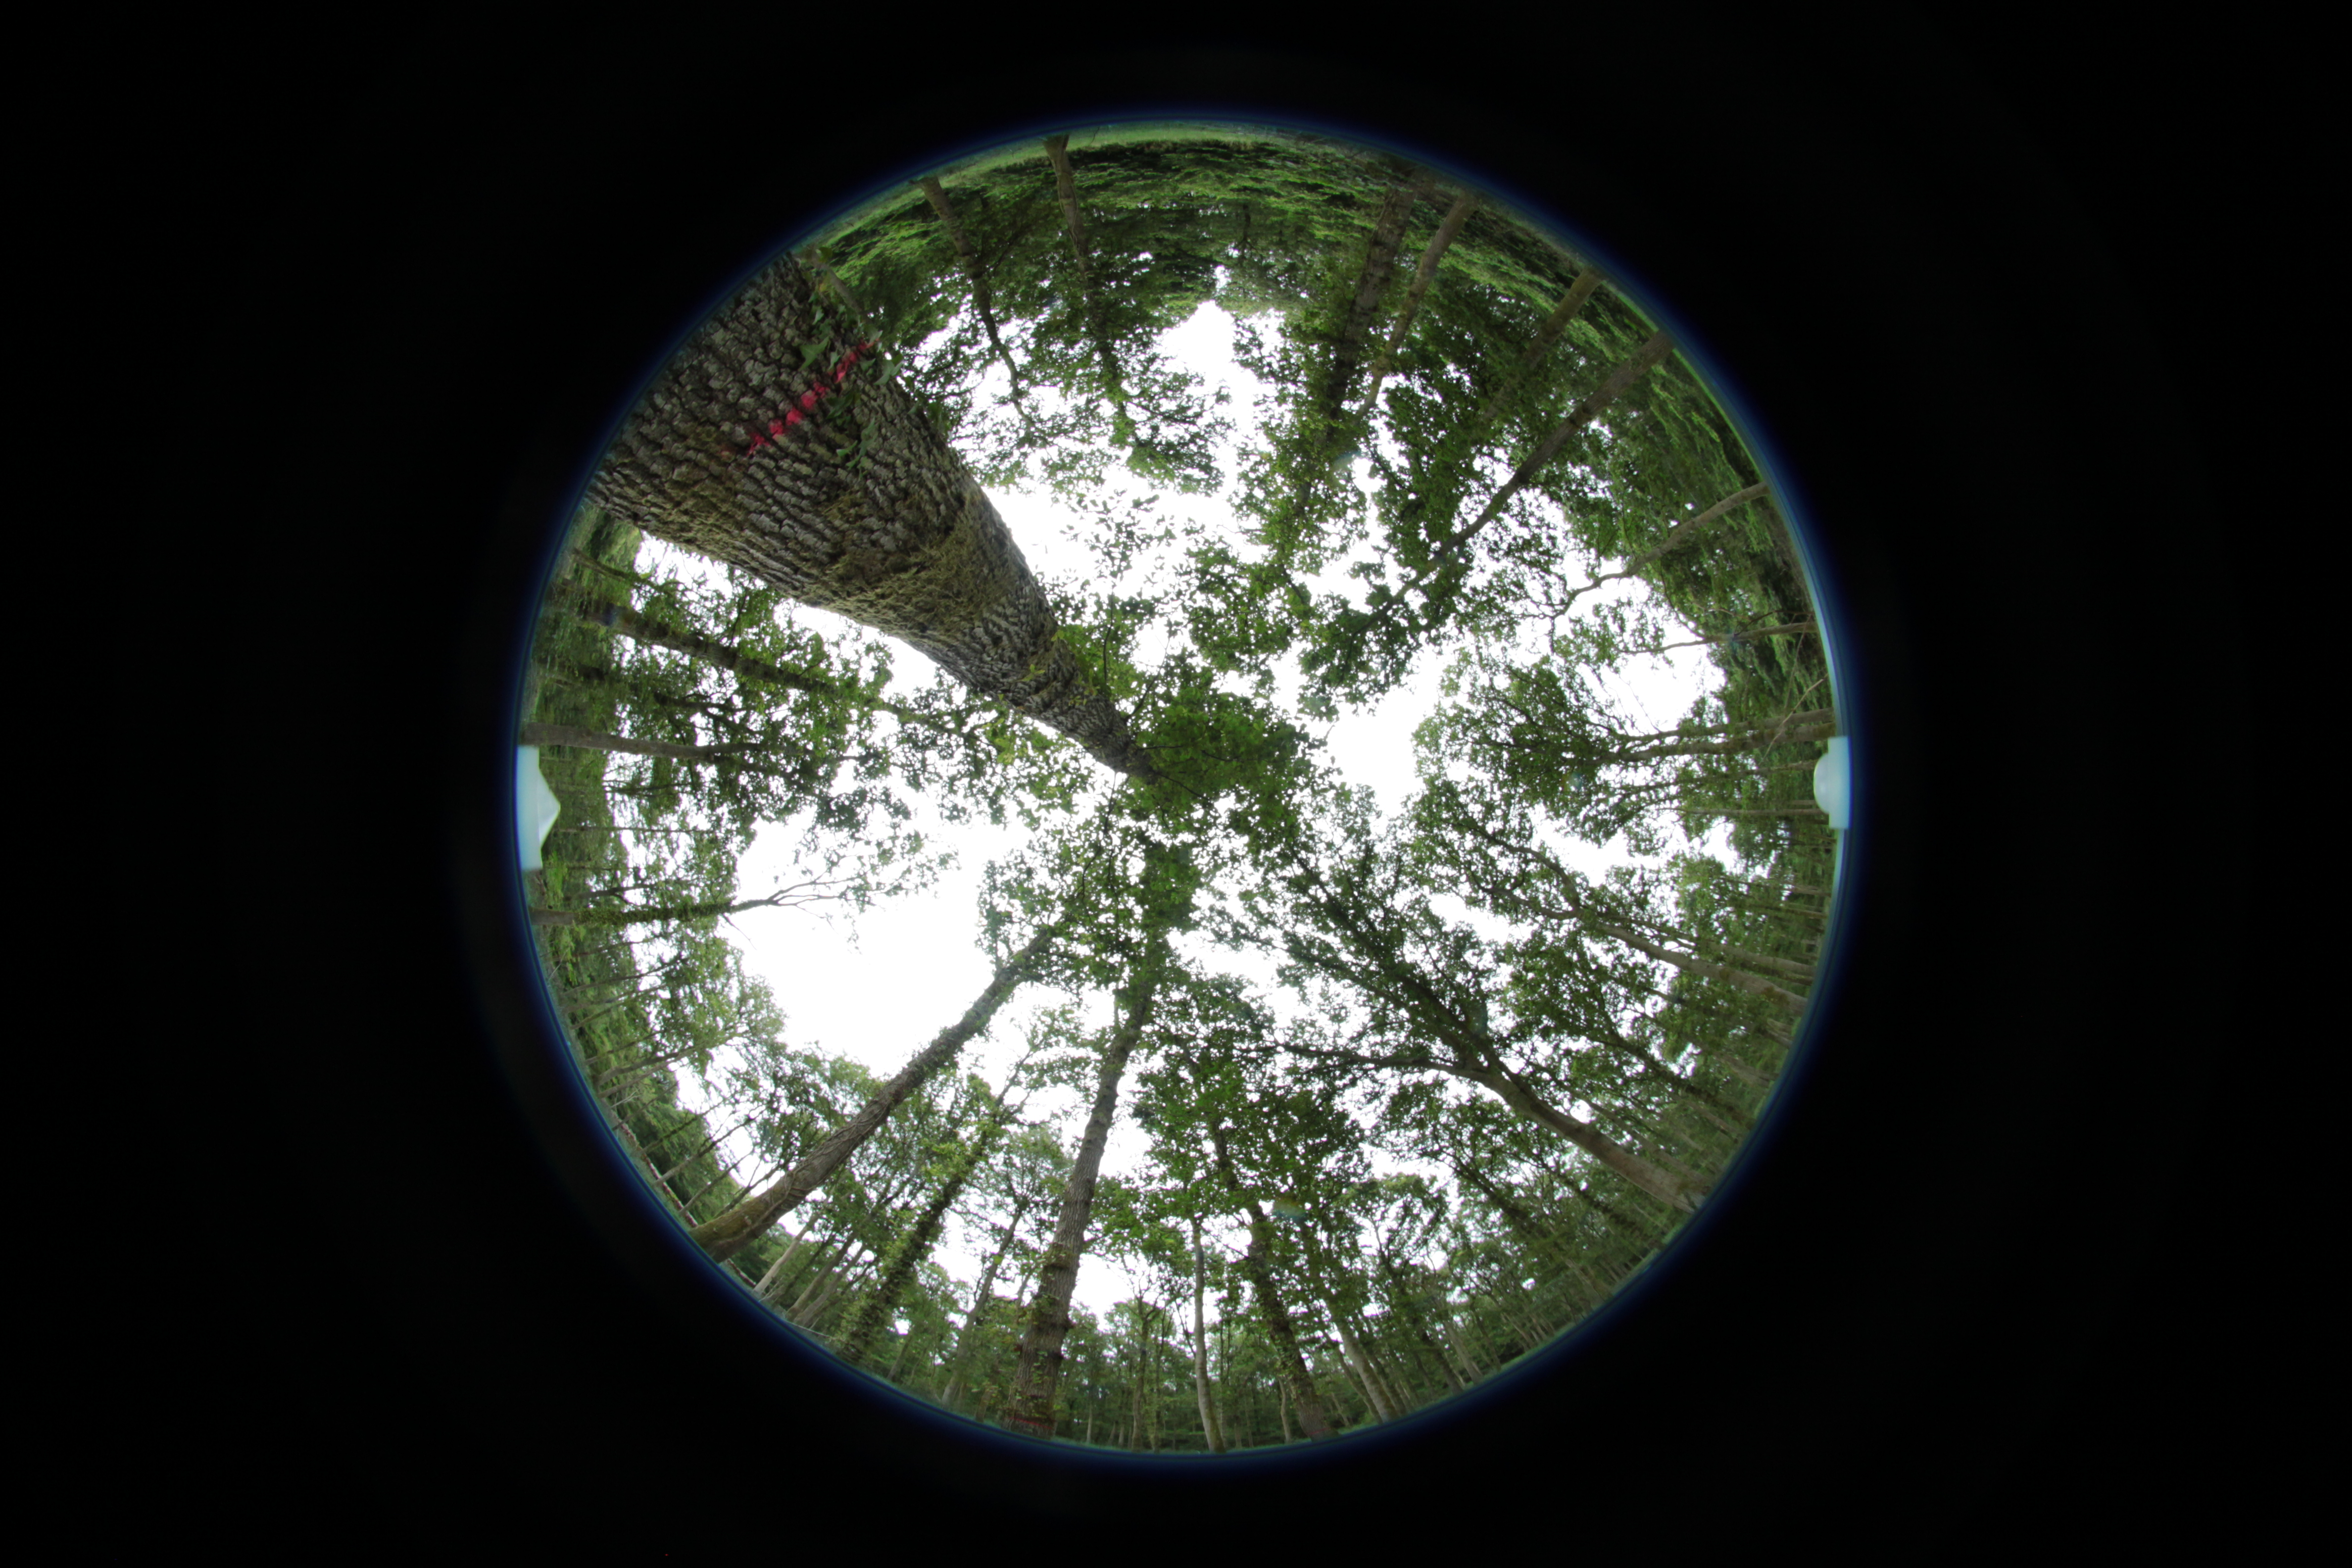
\includegraphics[width=.9\linewidth]{252exp1.jpg}
  \caption{Thinned}
  \label{fig:sub2}
\end{subfigure}
\caption{Hemispherical photographs from the Alice Holt flux site showing the difference between the thinned and unthinned sides of the forest.}
\label{fig:hemiphotos}
\end{figure}

\subsection{Litter traps}

\subsection{Comparison of methods}

\section{Point-centred quater observations}

\section{Flux tower observations and data processing}

\bibliography{../PhD}{}
\end{document}